\documentclass[t]{beamer}
\usetheme[english]{KIT}

\usepackage{amssymb} %% For \backprime
\usepackage{multicol}
\usepackage{mathpartir}

%\usepackage{mathpartir}
\usepackage{graphicx}

\usepackage{tikz}
\usetikzlibrary{arrows.meta,positioning,calc}

\usepackage[T1]{fontenc}
\usepackage{babel}
\usepackage{booktabs}
\usepackage[normalem]{ulem}
\usepackage{fontspec}
\setmonofont[RawFeature=-calt,Scale=MatchLowercase]{Iosevka}
%\newfontfamily\lc[Scale=MatchLowercase]{Iosevka SS09}

\usepackage{minted}
\definecolor{codebg}{rgb}{0.95,0.95,0.95}
\setminted{bgcolor=codebg,breaklines}
\usemintedstyle{tango}
\newmintinline[lean]{theorem.py:LeanLexer -x}{bgcolor=white}
\newminted[leancode]{theorem.py:LeanLexer -x}{fontsize=\footnotesize}

\usepackage{newunicodechar}
\newfontfamily{\freeserif}{DejaVu Sans}
\newunicodechar{ℕ}{\freeserif{ℕ}}
\newunicodechar{ℝ}{\freeserif{ℝ}}
\newunicodechar{ₐ}{\freeserif{ₐ}}
%\newunicodechar{₁}{\freeserif{₁}}
%\newunicodechar{∈}{\freeserif{∈}}
\newunicodechar{𝓞}{\ensuremath{\mathcal{O}}}
\newunicodechar{∉}{\freeserif{∉}}
%\newunicodechar{Π}{\freeserif{Π}}
%\newunicodechar{→}{\freeserif{→}}
\newunicodechar{⦃}{\freeserif{⦃}}
\newunicodechar{⦄}{\freeserif{⦄}}
%\newunicodechar{∧}{\freeserif{∧}}
%\newunicodechar{∨}{\freeserif{∨}}
%\newunicodechar{⊢}{\freeserif{⊢}}
\newunicodechar{⊑}{\freeserif{⊑}}
\newunicodechar{ₚ}{\freeserif{ₚ}}
\newunicodechar{∘}{\freeserif{∘}}
\newunicodechar{ₗ}{\freeserif{ₗ}}
\newunicodechar{∪}{\freeserif{∪}}
\newunicodechar{⋃}{\freeserif{⋃}}
\newunicodechar{𝓸}{\ensuremath{o}}
\newunicodechar{⊆}{\freeserif{⊆}}
\newunicodechar{≼}{\freeserif{≼}}
\newunicodechar{≃}{\freeserif{≃}}
\newunicodechar{✝}{\freeserif{✝}}

% https://github.com/gpoore/minted/issues/220
\AtBeginEnvironment{snugshade*}{\vspace{-0.4\FrameSep}}
%\AfterEndEnvironment{snugshade*}{\vspace{-0.8\FrameSep}}

% https://tex.stackexchange.com/questions/343494/minted-red-box-around-greek-characters
%\makeatletter
%\AtBeginEnvironment{minted}{\dontdofcolorbox}
%\def\dontdofcolorbox{
\renewcommand\fcolorbox[4][]{#4}
%}
%\makeatother

\title{Metaprogramming in Lean 4}

\author[Ullrich, de Moura]{Leonardo de Moura\inst{1}, Sebastian Ullrich\inst{2}}
\subtitle{\insertauthor}
 %\institute[IPD Snelting]{Programming paradigms group - IPD Snelting}
\institute[]{\inst{1}Microsoft Research, USA\ \ \ \inst{2}KIT, Germany}
\date{2021/01/06}
\makeatletter
\sbox{\KIT@titimg}{
  \hspace{0.08\titleimagewd}
    \raisebox{0.1\titleimageht}{
      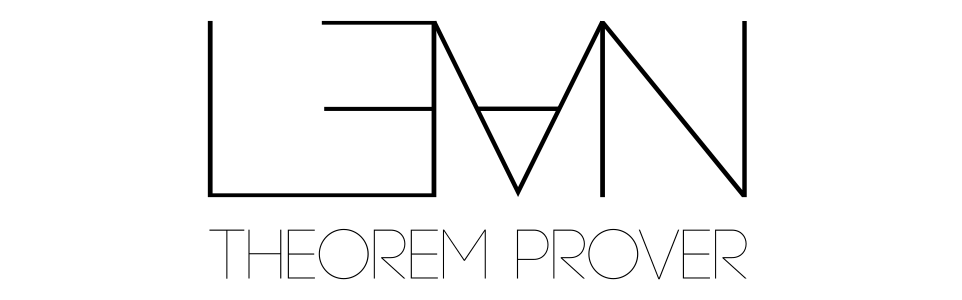
\includegraphics[height=0.8\titleimageht]{logo}
    }
}

\newcommand{\kit}[1]{\textcolor{KITgreen}{#1}}

\begin{document}
\begin{frame}
  \maketitle
\end{frame}

\begin{frame}[fragile]{The Lean 4 Frontend Pipeline}
  \begin{itemize}
  \item parser: \lean{≈ String → Syntax}
  \item macro expansion: \lean{Syntax → MacroM Syntax}
    \begin{itemize}
    \item actually interleaved with elaboration
    \end{itemize}
  \item elaboration
    \begin{itemize}
    \item terms: \lean{Syntax → TermElabM Expr}
    \item commands: \lean{Syntax → CommandElabM Unit}
    \item universes: \lean{Syntax → TermElabM Level}
    \item tactics: \lean{Syntax → TacticM Unit}
    \end{itemize}
    \pause
  \item pretty printer
    \begin{itemize}
    \item delaborator: \lean{Expr → DelaboratorM Syntax}
    \item parenthesizer: \lean{Syntax → ParenthesizerM Syntax}
    \item formatter: \lean{Syntax → FormatterM Format}
    \end{itemize}
  \end{itemize}
\end{frame}

\begin{frame}[fragile]{Notations}
\begin{leancode}
infixl:65 " + "  => HAdd.hAdd  -- left-associative
infix:65  " - "  => HSub.hSub  -- ditto
infixr:80 " ^ "  => HPow.hPow  -- right-associative
prefix:100 "-"   => Neg.neg
postfix:max "⁻¹" => Inv.inv
\end{leancode}
  \pause
  These are just macros.
\begin{leancode}
notation:65 lhs " + " rhs:66 => HAdd.hAdd lhs rhs
notation:65 lhs " - " rhs:66 => HSub.hSub lhs rhs
notation:70 lhs " * " rhs:71 => HMul.hMul lhs rhs
notation:80 lhs " ^ " rhs:80 => HPow.hPow lhs rhs
notation:100 "-" arg:100 => Neg.neg arg
notation:1000 arg "⁻¹" => Inv.inv arg
\end{leancode}
  \pause
\begin{leancode}
set_option trace.Elab.command true in
...
\end{leancode}
\end{frame}

\begin{frame}[fragile]{Mixfix Notations}
\begin{leancode}
notation:max "(" e ")" => e
notation:10 Γ " ⊢ " e " : " τ => Typing Γ e τ
\end{leancode}
  No other ``special'' forms of \lean{notation}
  \pause
\begin{leancode}
notation:65 a " + " b:66 " + " c:66 => a + b - c
#eval 1 + 2 + 3  -- 0
\end{leancode}
  Overlapping notations are parsed with a (local) ``longest parse'' rule
\end{frame}

\begin{frame}[fragile]{Syntax}
\begin{leancode}
notation:max "(" e ")" => e
\end{leancode}
  This is just a macro.
\begin{leancode}
syntax:max "(" term ")" : term
macro_rules
| `(($e)) => `($e)
\end{leancode}
  \lean{term} is a \emph{syntax category}
  \pause
\begin{leancode}
declare_syntax_cat index
syntax term : index
syntax term "≤" ident "<" term : index
syntax ident ":" term : index

syntax "{" index " | " term "}" : term
\end{leancode}
\end{frame}

\begin{frame}[fragile]{More Syntax}
\begin{leancode}
syntax binderIdent                := ident <|> "_"
syntax unbracketedExplicitBinders := binderIdent+ (" : " term)?

syntax "begin " tactic,*,? "end" : tactic
\end{leancode}
\end{frame}

\begin{frame}[fragile]{Lower-Level Syntax in \lean{Lean}}
\begin{leancode}
def fromTerm := parser! " from " >> termParser
@[builtinTermParser] def «show» := parser!:leadPrec "show " >> termParser >> (fromTerm <|> byTactic)
\end{leancode}
  is roughly equivalent to
\begin{leancode}
syntax fromTerm := " from " term
syntax:leadPrec "show " term (fromTerm <|> byTactic) : command
\end{leancode}
\end{frame}

\begin{frame}{Summary: Parsing}
  Each syntax category is
  \begin{itemize}
  \item a precedence (Pratt) parser composed of a set of leading and trailing parsers
  \item with per-parser precedences
  \item following the longest parse rule
  \end{itemize}

  \pause\bigskip

  on the lower level: a combinatoric, non-monadic, lexer-less, memoizing recursive-descent parser

  \url{https://github.com/leanprover/lean4/blob/master/src/Lean/Parser/Basic.lean\#L7}
\end{frame}

\begin{frame}[fragile]{Macros}
\AfterEndEnvironment{snugshade*}{\vspace{-0.2\FrameSep}}
\begin{leancode}
notation:max "(" e ")" => e
\end{leancode}
  This is just a macro.
\begin{leancode}
syntax:max "(" term ")" : term
macro_rules
| `(($e)) => `($e)
\end{leancode}
  \pause which can also be written as
\begin{leancode}
macro:max "(" e:term ")" : term => `($e)
\end{leancode}
  \pause or, in this case
\begin{leancode}
macro:max "(" e:term ")" : term => pure e
\end{leancode}
  \pause since it's really just
\begin{leancode}
  @[macro «term(_)»] def myMacro✝ : Macro✝
    | `(($e)) => pure e
    | _       => throw✝ Macro.Exception.unsupportedSyntax✝
\end{leancode}
\AfterEndEnvironment{snugshade*}{\vspace{0.2\FrameSep}}
\end{frame}

\begin{frame}[fragile,fragile,fragile]{Macros}
  Macros are extensible
\begin{leancode}
syntax ident "|" term : index
macro_rules
| `(_big [$op, $idx] ($i:ident | $p) $F) => `(bigop $idx (Enumerable.elems _) (fun $i:ident => ($i:ident, $op, $p, $F)))
#check Σ i | myPred i => i+i
#check Π i | myPred i => i+i
\end{leancode}
  (\emph{Beyond Notations} supplement, \url{https://github.com/leanprover/lean4/blob/master/tests/lean/run/bigop.lean})

\pause \bigskip
The newest macro is tried first, absent specific priorities
\begin{leancode}
macro (priority := high) ...
\end{leancode}
\end{frame}

\begin{frame}[fragile,fragile]{Quotations}
\begin{leancode}
`(let $id:ident $[$binders]* $[: $ty?]? := $val; $body)
\end{leancode}
  \vspace{-2\FrameSep}
  \begin{itemize}
  \item has type \lean{Syntax} in patterns
  \item has type \lean{m Syntax} given \lean{MonadQuotation m} in terms
  \item \lean{id}, \lean{val}, \lean{body} have type \lean{Syntax}
  \item \lean{binders} has type \lean{Array Syntax}
  \item \lean{ty?} has type \lean{Option Syntax}
    \pause
  \item \lean{ts} in \lean{$ts,*} has type \lean{SepArray}
  \end{itemize}
  \pause\bigskip
  \lean{syntax foo := ...} introduces a new \emph{antiquotation kind} \lean{$e:foo}

  \lean{declare_syntax_cat index} introduces a new antiquotation kind \lean{$e:index} and a new \emph{quotation kind} \lean{`(index|...)}
\end{frame}

\begin{frame}[fragile,fragile]{Scope of Hygiene}
\begin{leancode}
macro "foo" : term => do
  let a ← `(rfl)
  `(fun rfl => $a)
\end{leancode}
  \pause This unfolds to the identity function. Hygiene works \emph{per-macro}
 
  \pause\bigskip Nested scopes can be opened with \lean{withFreshMacroScope}

\begin{leancode}
def expandMatchAltsIntoMatchAux (matchAlts : Syntax) (discrs : Array Syntax) :
  Nat → MacroM Syntax
  | 0   => `(match $[$discrs:term],* with $matchAlts:matchAlts)
  | n+1 => withFreshMacroScope do
    let x ← `(x)
    let body ← expandMatchAltsIntoMatchAux matchAlts n (discrs.push x)
    `(@fun $x => $body)
\end{leancode}
\end{frame}

\begin{frame}{Summary: Macros}
  Macros are syntax-to-syntax translations
  \begin{itemize}
  \item applied iteratively and recursively
  \item associated with a specific parser and tried in a specific order
  \item with ``well-behaved'' (hygienic) name capturing semantics
  \end{itemize}
\end{frame}

\end{document}

%%% Local Variables:
%%% mode: latex
%%% TeX-master: t
%%% TeX-engine: xetex
%%% TeX-command-extra-options: "-shell-escape"
%%% End:
